\lstset{inputencoding=utf8x, extendedchars=false, keepspaces = true,
language=C++,
keywords={include, const, virtual, template, typename, class, private, public, operator, if, while, else, return, new, delete, int, float, bool, char},
sensitive=true,
%basicstyle=\small,
commentstyle=\scriptsize\rmfamily,
keywordstyle=\ttfamily\underbar,
identifierstyle=\ttfamily,
basewidth={0.5em,0.5em},
columns=fixed,
fontadjust=true,
breaklines=true,
literate={->}{{$\to$}}1
}

\title{Пользовательский уровень\\
библиотеки неконсервативной\\ 
сборки мусора\\
для C++}
%
\titlerunning{Библиотека неконсервативной сборки мусора для С++}
\author{Крень Мария Владимировна}
%
\authorrunning{М.В.Крень} % abbreviated author list (for running head)
%
%%%% list of authors for the TOC (use if author list has to be modified)
\tocauthor{М.В.Крень}
%
\institute{Санкт-Петербургский государственный университет\\
\email{mari.kren@gmail.com}}

\maketitle              % typeset the title of the contribution

\section*{Введение}

Динамическая память является одним из самых важных ресурсов, которым может распоряжаться программа. Использование
динамической памяти позволяет добиться выской гибкости и масштабируемости реализации, а также повысить уровень
абстракции и переиспользования кода. С другой стороны, использование динамической памяти ``вручную'' с помощью
примитивов низкого уровня может приводить к трудно обнаруживаемым, отложенным и редко проявляющимся ошибкам. 
Безопасное управление динамической памятью является одной из самых важных задач прикладного и системного программирования. 
Поэтому автоматизация управления динамической памятью~--- актуальная задача, решение которой так или иначе необходимо при
разработке многих современных языков программирования и окружающего их инструментария.

Одним из наиболее универсальных способов автоматического управления динамической памятью является \emph{сборка мусора} 
(garbage collection)~\cite{GCBook}. Суть сборки мусора заключается в том, что выделенная в приложении память, 
которая ему в дальнейшем не понадобится, освобождается системой управления памятью автоматически. Для этого в 
определённые моменты запускается процесс, самостоятельно освобождающий те участки памяти, до которых невозможно
добраться, используя ссылки, с которыми в данных момент работает программа.
 
Впервые сборка мусора была применена еще  в 1959 году Джоном Маккарти. Он использовал ее в среде программирования для 
разработанного им языка функционального программирования Lisp\footnote{\url{http://www.gnu.org/software/emacs/manual/html\_node/elisp/Garbage-Collection.html}}.
Вначале сборку мусора стали применять преимущественно в функциональных и логических языках, поскольку в таких языках затруднено
отслеживание времени жизни объектов в памяти. В промышленных процедурных и объектно-ориентированных языках технология сборки мусора стала 
приобретать популярность лишь со второй половины 1980-х годов. До этого времени ручное управление памятью считалось предпочтительнее как более 
эффективное и предсказуемое. Со второй половины 1990-х годов все чаще и чаще механизм сборки мусора включают в языки и среды, ориентированные 
на прикладное программирование. После появления языка программирования Java\footnote{\url{https://www.java.com/ru}} в 1995 году 
сборка мусора стала настоящим ``мейнстримом''.  На данный момент технология сборки мусора используется в таких языках, как Java, C\#, 
Python, Ruby, Perl и многих других. 

Сборка мусора обладает как достоинствами, так и недостатками. По сравнению с ручным управлением, автоматическое 
управление памятью безопаснее: программисту не нужно заботиться о том, когда освобождать память из-под объектов. 
Это дает гарантию того, что не возникнет некоторых ошибок, таких как висячий указатель, т.е. указатель на уже 
освобожденный объект, или ошибка повторного освобождения памяти, когда программа пытается освободить память, 
которая уже была освобождена.

С другой стороны при использовании сборки мусора могут возникнуть следующие проблемы:

\begin{enumerate}
\item если на объект есть ссылки из других достижимых объектов, то он никогда не будет удален;
\item во время работы программы из-за запуска сборщика мусора возникают паузы в непредвиденные моменты времени, а их 
продолжительность не определена.
\end{enumerate}

Для того, чтобы сборка мусора была возможна, должны выполняться определенные условия. Во-первых, должна присутствовать 
возможность определить все указатели из любого объекта на другие элементы кучи. Во-вторых, не должно быть никаких 
операций над указателями (логических, арифметических и т.п.) Часть из этих условий может быть автоматически выполнена
для некоторых языков (например, языков, в которых нет явного понятия указателя), выполнение остальных должно быть
обеспечено компилятором и библиотекой поддержки времени исполнения. Если это по каким-то причинам невозможно, то, строго
говоря, невозможна и надежная сборка мусора в общем случае. Тем не менее даже тогда можно добиться правильной
работы сборщика мусора, если каким-то образом ограничить вид программ, для которых он запускается. Такой подход применяется 
в ситуации, когда требуется использовать сборку мусора для тех языков, для которых она невозможна (или труднореализуема) 
в общем случае. Таким языком, например, является С++.

Язык С++~--- один из самых развитых и распространенных универсальных языков программирования. Свою популярность он приобрел 
благодаря гибкости, пригодности для реализации широкого класса задач и эффективности кода, порождаемого его 
компиляторами. Однако оборотной стороной этих его достоинств является то, что он по принципиальным соображениям не 
совместим со сборкой мусора, поскольку содержит низкоуровневые конструкции оперирования с памятью (указатели, адресную 
арифметику, неконтролируемые приведения типов). Тем не менее широкий класс прикладных программ может обойтись без этих
низкоуровневых возможностей, поэтому для него существуют библиотечные инструменты, позволяющие автоматизировать
управление динамической памятью при соблюдении определенных соглашений. В данной работе описывается
библиотека, независимая от конкретного компилятора, применение которой позволяет использовать в прикладной
программе на С++ точную сборку мусора.
\section{Некоторые средства автоматизации\\
управления памятью для С++}

Одним из наиболее широко используемых средств автоматизации управления памятью в
контексте языка С++ являются ``умные указатели'' (smart pointers). ``Умный указатель''~---
это специальный объект, который хранит указатель на участок динамически отведенной области
памяти и определяет некоторую дисциплину обращения с этом указателем. Иногда следование
этой дисциплине является лишь соглашением, и тогда ``умный указатель'' является всего лишь
способом идентифицировать необходимость правильного обращения с данными; однако довольно часто
``умные указатели'' действительно определенным образом ограничивают набор возможных
способов манипулирования данными за счет использования декларативных возможностей языка С++.

Простейший ``умный указатель'' может выглядеть так:

\begin{lstlisting}[language=C++,mathescape=true]
    template <typename T> class smart_pointer {
      T *m_obj; // $\mbox{Указатель на динамические данные}$
      public:
        // $\mbox{Конструктор получает исходный указатель}$
        smart_pointer (T *obj) : m_obj(obj) {}
        // $\mbox{Деструктор удаляет адресуемые данные}$
        ~smart_pointer () { delete m_obj; }
        // $\mbox{Перегруженные операторы для обращения к данным}$
        T* operator-> () { return m_obj; }
        T& operator*  () { return *m_obj; }
    }
\end{lstlisting}

Такой указатель позволяет обеспечить автоматическое освобождение области динамической памяти, если 
время её жизни можно ограничить временем жизни самого ``умного указателя''. При этом никак не
контролируется, что сам ``умный указатель'' используется правильно --- например, что конструктор
получает действительно адрес в куче или что для данного адреса создан только один ``умный указатель''.

Другим примером ``умного указателя''является \lstinline{Boost::scoped_ptr}\footnote{\url{http://www.boost.org/doc/libs/1\_39\_0/libs/smart\_ptr/scoped\_ptr.htm}} 
библиотеки BOOST\footnote{\url{http://www.boost.org}}. Его основное отличие от приведенного выше~--- отсутствие возможности копирования и присваивания (а,
значит, и передачи параметром в функцию). Эти ограничения не исключают возможность неправильного использования, но позволяют избежать некоторых из них.

Еще одним вариантом является \lstinline{auto_ptr}\footnote{\url{http://www.cplusplus.com/reference/memory/auto\_ptr}}. Этот указатель разрешает
операции копирования и передачи параметром, но при этом ``опустошается'' содержимое источника. Таким образом, указатели не копируются, 
а ``перемещаются'', что позволяет избежать ситуации, когда происходит несколько попыток освободить одну и ту же область памяти из-за хранения 
её адреса разными ``умными указателями''. С другой стороны, теперь не гарантируется, что ``умный указатель'' всегда указывает на правильные данные ---
в какой-то момент он может ``испортиться''. В силу этого такие указатели нельзя использовать в контейнерах STL. Для таких целей используются
\lstinline{std::shared_ptr}.

\lstinline{shared_ptr}\footnote{\url{http://www.cplusplus.com/reference/memory/shared\_ptr}}~--- это ``умный указатель'' с подсчетом ссылок. Это значит, 
что с каждой областью памяти, адресуемой \lstinline{shared_ptr}, ассоциирована переменная, которая хранит количество указателей, которые ссылаются на начало
этой области памяти. Если эта переменная становится равной нулю, то область освобождается. Счетчик инкрементируется при каждом вызове оператора копирования 
или оператора присваивания. У \lstinline{shared_ptr} есть оператор приведения к типу \lstinline{bool}, что позволяет проверять, указывает ли он на что-нибудь.
Использование \lstinline{shared_ptr} может обеспечить сравнительно безопасную автоматизацию управления памятью, однако неприятности все же возможны. Во-первых,
наличие указателя \lstinline{shared_ptr} не на начало динамически отведенной области памяти не гарантирует её сохранения; кроме того, циклические
ссылки приводят к образованию неудаляемого мусора; наконец, возможна ситуация лавинообразного освобождения памяти с возникновением непредсказуемой
задержки.

\section{Используемые особенности языка С++}

Реализация сборки мусора в виде внешней библиотеки существенно опирается 
на некоторые особенности как языка С++, так и его компиляторов и среды поддержки времени 
исполнения. К таковым особенностям относятся:

\begin{enumerate}
\item функция \lstinline{typeid} и возможность идентификации типа во время исполнения (runtime type identification, RTTI);
\item инициализация по размещению (placement new);
\item шаблоны, в том числе шаблоны с переменным числом аргументов (templates, variadic templates);
\item конструкторы, деструкторы и порядок их вызова.
\end{enumerate}

Далее рассмотрим вышеперечисленные особенности подробнее.

\subsection{Функция \lstinline{typeid} и идентификация типа\\
во время исполнения} 

Идентификация типа во время исполнения позволяет получить метаинформацию о типе объекта во время работы программы. 
В сборщике мусора эта метаинформация используется для установления связи между объектом и метаинформацией сборщика
мусора, соответствующей этому типу. Для того, чтобы это стало возможно, поддержка RTTI должна быть включена 
соответствующими опциями компилятора.

На пользовательском уровне возможности RTTI представлены функцией \lstinline{typeid}\footnote{\url{http://www.c-cpp.ru/books/identifikaciya-tipa-vo-vremya-ispolneniya-rtti}},
которая получает указатель на объект и возвращает ссылку на объект типа \lstinline{typeinfo}. Данный тип
содержит информацию о типе объекта, в частности, имя этого типа, которое и используется в сборщике мусора.

\subsection{Инициализация по размещению, шаблоны,\\
шаблоны с произвольным числом аргументов} 

Инициализация по размещению и шаблоны с произвольным числом аргументов в реализации сборщика мусора используются 
совместно для того, чтобы выразить примитив выделения памяти. Основная задача, которая при этом возникает 
кроме собственно выделения~--- определение типа объекта, занимающего данную область памяти, и её аннотирование
соответствующей метаинформацией. 

Отследить момент выделения памяти можно было бы путем перегрузки глобального оператора \lstinline{new}; однако
в этом случае было бы трудно узнать, каков тип объекта, для которого выделяется память. Использование же
инициализации по размещению, шаблонов и шаблонов с произвольным числом аргументов позволяет инкапсулировать
всю нужную функциональность в одной функции, которая отведет память, вызовет конструктор, передав
ему нужное количество аргументов, и кроме того выполнит все остальные необходимые действия.

 \subsection{Конструкторы, деструкторы и порядок их вызова} 

Важным фактом является то, что в С++ момент создания/удаления объекта можно отследить с помощью 
конструктора/деструктора\footnote{\url{http://www.developerfusion.com/article/133063/constructors-in-c11/}}. 
В сборщике мусора это используется для того, чтобы, во-первых, построить метаинформацию для данного типа (каждый
``умный указатель'' при создании регистрирует себя в некоторой структуре данных) и, во-вторых, чтобы регистрировать
корневые указатели во внешнем пуле корней.

\section {Пользовательский уровень библиотеки\\
сборки мусора}

С точки зрения пользователя библиотека сборки мусора представлена одним шаблонным классом
``умного указателя'' 

\begin{lstlisting}
    template <class T> class gc_ptr {
       ...
    }
\end{lstlisting}

и одной шаблонной функцией выделения памяти

\begin{lstlisting}
    template <class T, typename ... Types> T* gc_new (
    Types ... types, size_t count = 1
    ) {
       ...
    }
\end{lstlisting}

которые становятся доступными после подключения одного заголовочного файла:

\begin{lstlisting}
    # include <libgc/libgc.h>
\end{lstlisting}

Исполняемый код библиотеки содержится в модулях, которые могут быть как собраны статически вместе
с приложением, так и подгружены динамически.

Любая программа, которая в качестве примитива выделения памяти использует \lstinline{gc_new}, в качестве
указателей --- \lstinline{gc_ptr}, и не содержит явного освобождения памяти с помощью \lstinline{delete}, будет
работать с использованием сборки мусора.

Семантика описанных примитивов с точки зрения сборки мусора будет описана в следующем разделе; пока же
мы обсудим их интерфейс с точки зрения пользователя.

\subsection{Интерфейс \lstinline{gc_ptr}}

Класс \lstinline{gc_ptr} инкапсулирует всю функциональность указателя, которая безопасна с точки зрения
сборки мусора. Данный класс реализует следующие операторы:

\begin{enumerate}
\item \lstinline{T& operator*() const}~--- разыменование;
\item \lstinline{T* operator->() const, operator T* () const}~--- доступ к указателю;
\item \lstinline{T& operator[](size_t index)}~--- доступ к элементам массива;
\item \lstinline{bool operator== (const gc_ptr <T> &a), bool operator== (const T* a)}~--- проверки на равенство;
\item \lstinline{bool operator!= (const gc_ptr <T> &a), bool operator!= (const T* a)}~--- проверки на неравенство;
\item \lstinline{gc_ptr& operator = (const gc_ptr <T> &a), gc_ptr& operator = (T* a)}~--- присваивание.
\end{enumerate}

Кроме того, у данного класса два конструктора: \lstinline{gc_ptr (T* p)} и \lstinline{gc_ptr (const gc_ptr <T> &p)}. 

\subsection{Функция выделения памяти \lstinline{gc_new}}

В языке С++ существует пять различных вариантов выделения памяти с помощью оператора \lstinline{new}. 
Этот оператор пытается выделить достаточно памяти в куче для размещения новых данных и, в случае успеха, возвращает 
адрес выделенного участка. После выделения памяти вызывается конструктор создаваемого объекта. Однако, если оператор
\lstinline{new} не может выделить память в куче, то возбуждается исключение типа \lstinline{std::bad_alloc}. 

Функция \lstinline{gc_new} позволяет выразить все ситуации, в которых может быть употреблён оператор \lstinline{new}.
Ниже мы приведем примеры использования \lstinline{gc_new} в каждой из них.

\begin {enumerate}
\item \lstinline{gc_new<type> ()}~--- выделение памяти под значение атомарного типа (\lstinline{int}, \lstinline{float} и т.д.); 
\item \lstinline{gc_new<C> ()}~--- выделение памяти под одиночный экземпляр объект класса \lstinline{C} с вызовом конструктора по
умолчанию;
\item \lstinline{gc_new <type> (len)}~--- выделение памяти под массив длины \lstinline{len} из элементов атомарного типа \lstinline{type};
\item \lstinline{gc_new <C> (len)}~--- выделение памяти под массив длины \lstinline{len} из экземпляров класса \lstinline{C}, для каждого из
которых вызывается конструктор по умолчанию;
\item \lstinline{gc_new <C, T1, T2, ..> (a1, a2, ..)}~--- выделение памяти под экземпляр объекта класса \lstinline{C} с вызовом
конструктора с парамерами \lstinline{a1, a2, ..}, имеющими типы \lstinline{T1, T2, ..} соответственно.
\end {enumerate}

Таким образом примитив выделения памяти в языке С++ для объектов различных типов можно заменить вызовом функции \lstinline{gc_new} 
соответствующего вида.

\subsection{Пример использования пользовательских\\
примитивов}

В качестве примера использования пользовательских примитивов библиотеки сборки мусора приведем 
реализацию класса строк:

\begin{lstlisting}
    class GCString {
      private:
        gc_ptr<char> pData; 	
        int length;	 
        GCString (gc_ptr<char> p, int l) : pData (p), length (l) {};     
      public:
        GCString () : length (0), pData (NULL) {};
        GCString (const char *cString);
        virtual ~GCString () {};
        GCString (const GCString &s);
        GCString operator= (const GCString &s);
        GCString operator= (const char *cString);
        char operator[] (int i) {return pData [i];};
        GCString operator+  (const GCString &s);
        GCString operator+  (const char *cString);
        GCString operator+= (GCString& s);
      };

      GCString::GCString (const char *cString) {
        length = strlen (cString);
        pData  = gc_new<char> (length+1);
        strcpy ((char *) pData, cString);
      }

      GCString::GCString (const GCString &s) : 
        length (s.length), pData (s.pData) {}

      GCString GCString::operator= (const GCString &s) {
        length = s.length;
        pData  = s.pData;
        return *this;
      }

      GCString GCString::operator= (const char *cString) {
        return *this = GCString (cString);
      }

      GCString GCString::operator+ (const GCString &s) {
        gc_ptr<char> p = gc_new<char> (length + s.length + 1);
        strcpy (p, (char*) this->pData);
        strcat (p, (char*) s.pData);
        return GCString (p, length + s.length);
      }

      GCString GCString::operator+ (const char *cString) {
        return *this + GCString (cString);
      }

      GCString GCString::operator+= (GCString &s) {
        return *this = *this + s;
      }
\end{lstlisting}

\section{Семантика примитивов\\
пользовательского уровня\\
с точки зрения сборки мусора}

Одним из самых популярных алгоритмов сборки мусора является  алгоритм ``\emph{пометки и 
освобождения}'' (mark-and-sweep). Его популярность обусловлена простотой и тем, что 
данный алгоритм накладывает минимальные ограничения на организацию поддержки времени
исполнения и требует минимальной поддержки со стороны компилятора. 

Задачи, решаемые в процессе организации сборщика мусора такого типа, показаны на Рис.~1.

\begin{figure}[h!]
	\centering
	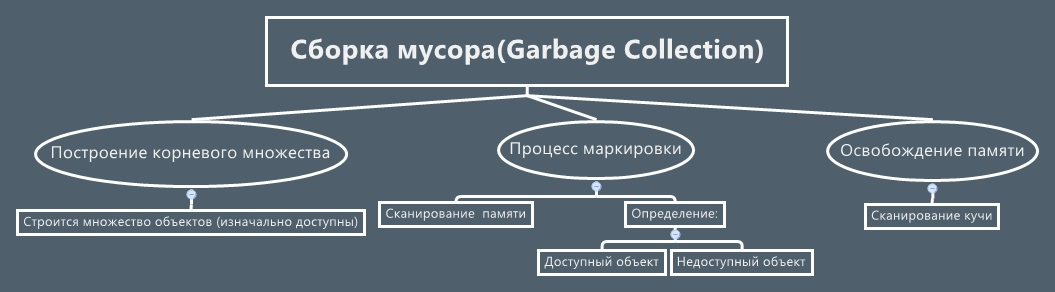
\includegraphics[width=500pt]{Kren/picture1.jpg}
	\caption{Три основных этапа сборки мусора}
	\centering
\end{figure}

Алгоритм ``пометки и освобождения'' состоит из двух фаз, которые запускаются последовательно
одна за другой:

\begin{itemize}
\item Фаза пометки. Начиная с некоторого аксиоматически заданного множества указателей, называемого
\emph{корневым множеством}, происходит полный обход всех достижимых объектов. Каждый достижимый
объект помечается как живой.
\item Фаза освобождения. Происходит полный обход кучи, во время которого освобождается память
из-подо всех непомеченных объектов; при этом пометка с помеченых объектов снимается.
\end{itemize}

Для реализации сборки мусора с помощью алгоритма ``пометки и освобождения'' должны быть решены
следующие задачи:

\begin{enumerate}
\item Идентификация корневого множества. Корневое множество~--- это множество указателей на
объекты, которые считаются изначально доступными для программы. Такие указатели хранятся в
стеке, регистрах и статической области памяти. В задачу идентификации корневого множества 
входит распознавание указателей в кучу на отведенные там объекты среди всех таких значений.

\item Определение всех ссылок из данного объекта на другие объекты в куче, что необходимо для
обхода всех достижимых объектов в фазе пометки.

\item Обеспечение возможности пометки объектов в куче и обхода всей кучи с освобождением 
непомеченных объектов.
\end{enumerate}

Последняя задача относится к реализации кучи; её решение изложено в~\cite{realisation}. Ниже 
мы опишем, как с помощью пользовательских примитивов, введенных в предыдущем разделе,
нами решаются две первые задачи.

\subsection{Поддержка корневого множества}

Идентификация корневого множества указателей (то есть указателей, хранящихся на стеке, в регистрах и статической
области памяти) без помощи со стороны компилятора является серьезной проблемой~\cite{roots}. При ``библиотечном''
подходе к сборке мусора рассчитывать на поддержку со стороны компилятора не приходится, поэтому в момент
начала сборки мусора идентифицировать корневые указатели уже невозможно. Поэтому корневое множество
поддерживается по мере работы программы. В него добавляются все \lstinline{gc_ptr}, экземпляры которых
не созданы с помощью \lstinline{gc_new}. Для этого в функции \lstinline{gc_new} выставляется флаг,
который проверяется в конструкторе \lstinline{gc_ptr}; в этом же конструкторе происходит добавление
указателя на объект \lstinline{gc_ptr} в пул корней, если это необходимо. Удаление же корневого
указателя происходит при вызове его деструктора. Так как удалять нужно только корневые указатели, а деструкторы
вызываются для всех, в \lstinline{gc_ptr} хранится признак того, что это корень. Поскольку деструкторы 
вызывается по отношению к конструкторам в обратном порядке (для автоматических объектов), пул корней можно 
реализовать в виде стека в отдельной области памяти вне кучи. 

\subsection{Построение метаинформации}

Представление метаинформации для сборки мусора, использованное нами, близко к тому, что описано
в~\cite{meta}. Метаинформация для типа представляет собой вектор смещений объектов \lstinline{gc_ptr} 
относительно начала экземпляра этого типа. Функция \lstinline{gc_new}, используемая для создания объектов, 
осуществляет поиск метаинформации по имени типа, полученному с помощью функции \lstinline{typeid}. 
Если этот поиск неуспешен (и, следовательно, для данного типа еще не была построена метаинформация), 
то создается новый объект, хранящий метаинформацию, и ассоциируется с именем этого типа. Для построения
метаинформации используются вызовы конструкторов \lstinline{gc_ptr}, с помощью которых можно
посчитать разность между адресом начала объекта и адресом, по которому ``внутри'' него расположен данный
\lstinline{gc_ptr}. 

После получения метаинформации функция \lstinline{gc_new} размещает указатель на неё перед данными 
создаваемого объекта. Это даёт возможность по указателю на живой объект узнать все указатели
из него на другие живые объекты, то есть реализовать стадию маркировки.

\section*{Заключение}

В результате выполнения данной работы были достигнуты следующие результаты:

\begin{enumerate}
\item изучены различные способы автоматизации управления памятью для языка C++ на 
основе использования ``умных указателей'';

\item разработан интерфейс библиотеки, позволяющей реализовать неконсервативную сборку мусора
при выполнении определенных соглашений на вид использующей её программы.

\item данное решение было использовано в рамках проекта по разработке библиотеки неконсервативной 
сборки мусора для языка С++;

\item полученная библиотека была протестирована на ряде примеров.
\end{enumerate}

\begin{thebibliography}{99}

\bibitem{GCBook} 
Richard Jones, Rafael Lins. Garbage Collection: Algorithms for Automatic Dynamic Memory Management. John Wiley \& Sons, 2001.

\bibitem{roots}
Д.А. Березун. Построение корневого множества указателей для сборки мусора // Труды лаборатории языковых инструментов JetBrains, 
выпуск 1. Санкт-Петербург, 2013.

\bibitem{meta}
М.В. Крень. Представление данных для сборки мусора // Труды лаборатории языковых инструментов JetBrains, выпуск 1. Санкт-Петербург, 2013.


\bibitem{realisation}
Д.А. Березун. Реализация основных примитивов библиотеки неконсервативной сборки мусора для С++ // настоящий сборник.

\bibitem{standart}
Bjarne Stroustrup. C++11 --- the new ISO C++ standard // \url{http://www.stroustrup.com/C++11FAQ.html}

\end{thebibliography}
